% ---------------------------------------------------------------------------
%                   LATEX TEMPLATE FOR MARL PhD THESIS
% ---------------------------------------------------------------------------

% Taemin Cho put together a nice LaTeX class, that Oriol Nieto modified.
% Eric Humphrey added all of this sweet content, and made it available to 
% the rest of MARLities.

% Everything is based on Harish Bhanderi's PhD/MPhil template, then Uni Cambridge
% http://www-h.eng.cam.ac.uk/help/tpl/textprocessing/ThesisStyle/
% corrected and extended in 2007 by Jakob Suckale, then MPI-CBG PhD programme
% and made available through OpenWetWare.org - the free biology wiki

%: Style file for Latex NYU-MARL:
% This template package can be found in ./Latex/Classes/
% It aims to follow the official NYU-Steinhardt guidelines:
%       http://steinhardt.nyu.edu/doctoral/dissertation/formatting
\documentclass[oneside, 12pt, letterpaper]{Latex/Classes/NYUdissertation}

%: Macro file for Latex
% Macros help you summarise frequently repeated Latex commands.
% Here, they are placed in an external file /Latex/Macros/MacroFile1.tex
% An macro that you may use frequently is the figuremacro (see introduction.tex)
% This file contains macros that can be called up from connected TeX files
% It helps to summarise repeated code, e.g. figure insertion (see below).

% insert a centered figure with caption and description
% parameters 1:filename, 2:title, 3:description and label
\newcommand{\figuremacro}[3]{
	\begin{figure}[htbp]
		\centering
		\includegraphics[width=1\textwidth]{#1}
		\caption[#2]{\textbf{#2} - #3}
		\label{#1}
	\end{figure}
}

% insert a centered figure with caption and description AND WIDTH
% parameters 1:filename, 2:title, 3:description and label, 4: textwidth
% textwidth 1 means as text, 0.5 means half the width of the text
\newcommand{\figuremacroW}[4]{
	\begin{figure}[htbp]
		\centering
		\includegraphics[width=#4\textwidth]{#1}
		\caption[#2]{\textbf{#2} - #3}
		\label{#1}
	\end{figure}
}

% inserts a figure with wrapped around text; only suitable for NARROW figs
% o is for outside on a double paged document; others: l, r, i(inside)
% text and figure will each be half of the document width
% note: long captions often crash with adjacent content; take care
% in general: above 2 macro produce more reliable layout
\newcommand{\figuremacroN}[3]{
	\begin{wrapfigure}{o}{0.5\textwidth}
		\centering
		\includegraphics[width=0.48\textwidth]{#1}
		\caption[#2]{{\small\textbf{#2} - #3}}
		\label{#1}
	\end{wrapfigure}
}

% predefined commands by Harish
\newcommand{\PdfPsText}[2]{
  \ifpdf
     #1
  \else
     #2
  \fi
}

\newcommand{\IncludeGraphicsH}[3]{
  \PdfPsText{\includegraphics[height=#2]{#1}}{\includegraphics[bb = #3, height=#2]{#1}}
}

\newcommand{\IncludeGraphicsW}[3]{
  \PdfPsText{\includegraphics[width=#2]{#1}}{\includegraphics[bb = #3, width=#2]{#1}}
}

\newcommand{\InsertFig}[3]{
  \begin{figure}[!htbp]
    \begin{center}
      \leavevmode
      #1
      \caption{#2}
      \label{#3}
    \end{center}
  \end{figure}
}


%%% Local Variables: 
%%% mode: latex
%%% TeX-master: "~/Documents/LaTeX/CUEDThesisPSnPDF/thesis"
%%% End: 


%: ----------------------------------------------------------------------
%:                  TITLE PAGE: name, degree,..
% ----------------------------------------------------------------------
% below is to generate the title page with crest and author name

%if output to PDF then put the following in PDF header
\ifpdf
    \pdfinfo { /Title  (Bear Claw Macaroon Tiramisu Cheesecake)
               /Creator (TeX)
               /Producer (pdfTeX)
               /Author (Your Name addy@nyu.edu)
               % /CreationDate (D:YYYYMMDDhhmmss)  %format D:YYYYMMDDhhmmss
               % /ModDate (D:YYYYMMDDhhmm)
               /Subject (Music Technology)
               /Keywords (Marzipan, jujubes, pudding, sesame snaps) }
         \pdfcatalog { /PageMode (/UseOutlines)
                  /OpenAction (fitbh)  }
\fi

\title{\doublespacing Bear Claw Macaroon Tiramisu Cheesecake}

\threecommittee
{Professor I.~M. Smart, Chairperson}
{Professor Beardsley Wordsworth}
{Professor Norma Hazelwood}

\degree{Doctor of Philosophy}
\degreedate{2014}

% ----------------------------------------------------------------------
% The section below defines www links/email for author and institutions
% They will appear on the title page of the PDF and can be clicked

%: ----------------------- HELP: www links
% You can also see below how, www links are placed
% \href{http://www.something.net}{link text}

\author{\href{mailto:addy@nyu.edu}{Your Name}}
\program{Program in \href{http://steinhardt.nyu.edu/music/technology/}{Music Technology}}
\department{Department of \href{http://steinhardt.nyu.edu/music/}{Music and Performing Arts Professions}}
\university{\href{http://www.nyu.edu/}{New York University}}
\crest{}%\includegraphics[width=3in]{NYUlogoLarge2597}}
\submittedtext{Submitted in partial fulfillment\\
  of the requirements for the degree of\\
  Doctor of Philosophy in the\\
  \href{http://steinhardt.nyu.edu/}{Steinhardt School of Culture, Education, and Human Development}}


% ----------------------------------------------------------------------

% turn of those nasty overfull and underfull hboxes
\hbadness=10000
\hfuzz=50pt
\makeindex

%:--------------------------------------------------------------
%:                  FRONT MATTER: dedications, abstract,..
% --------------------------------------------------------------

\begin{document}

%\hyphenpenalty=9000
%\frontmatter
\widowpenalty=10000
\clubpenalty=10000


%: ----------------------- generate cover page ------------------------
%\setstretch{1.2}
\maketitle  % command to print the title page with above variables
\makecopyright

%: ----------------------- abstract ------------------------

% Your institution may have specific regulations if you need an abstract and where it is to be placed in the document. The default here is just after title.

% 
% ----------------------------------------------------------------------
%                   LATEX TEMPLATE FOR PhD THESIS
% ----------------------------------------------------------------------

%: Style file for Latex
% Most style definitions are in the external file NYUdissertation
% In this template package, it can be found in ./Latex/Classes/

\documentclass[oneside, 12pt, letterpaper, nyustyle]{Latex/Classes/NYUdissertation}
%\documentclass[oneside, 12pt, letterpaper]{Latex/Classes/NYUdissertation}

%: Macro file for Latex
% Macros help you summarise frequently repeated Latex commands.
% Here, they are placed in an external file /Latex/Macros/MacroFile1.tex
% An macro that you may use frequently is the figuremacro (see introduction.tex)
% This file contains macros that can be called up from connected TeX files
% It helps to summarise repeated code, e.g. figure insertion (see below).

% insert a centered figure with caption and description
% parameters 1:filename, 2:title, 3:description and label
\newcommand{\figuremacro}[3]{
	\begin{figure}[htbp]
		\centering
		\includegraphics[width=1\textwidth]{#1}
		\caption[#2]{\textbf{#2} - #3}
		\label{#1}
	\end{figure}
}

% insert a centered figure with caption and description AND WIDTH
% parameters 1:filename, 2:title, 3:description and label, 4: textwidth
% textwidth 1 means as text, 0.5 means half the width of the text
\newcommand{\figuremacroW}[4]{
	\begin{figure}[htbp]
		\centering
		\includegraphics[width=#4\textwidth]{#1}
		\caption[#2]{\textbf{#2} - #3}
		\label{#1}
	\end{figure}
}

% inserts a figure with wrapped around text; only suitable for NARROW figs
% o is for outside on a double paged document; others: l, r, i(inside)
% text and figure will each be half of the document width
% note: long captions often crash with adjacent content; take care
% in general: above 2 macro produce more reliable layout
\newcommand{\figuremacroN}[3]{
	\begin{wrapfigure}{o}{0.5\textwidth}
		\centering
		\includegraphics[width=0.48\textwidth]{#1}
		\caption[#2]{{\small\textbf{#2} - #3}}
		\label{#1}
	\end{wrapfigure}
}

% predefined commands by Harish
\newcommand{\PdfPsText}[2]{
  \ifpdf
     #1
  \else
     #2
  \fi
}

\newcommand{\IncludeGraphicsH}[3]{
  \PdfPsText{\includegraphics[height=#2]{#1}}{\includegraphics[bb = #3, height=#2]{#1}}
}

\newcommand{\IncludeGraphicsW}[3]{
  \PdfPsText{\includegraphics[width=#2]{#1}}{\includegraphics[bb = #3, width=#2]{#1}}
}

\newcommand{\InsertFig}[3]{
  \begin{figure}[!htbp]
    \begin{center}
      \leavevmode
      #1
      \caption{#2}
      \label{#3}
    \end{center}
  \end{figure}
}


%%% Local Variables: 
%%% mode: latex
%%% TeX-master: "~/Documents/LaTeX/CUEDThesisPSnPDF/thesis"
%%% End: 


%: ----------------------------------------------------------------------
%:                  TITLE PAGE: name, degree,..
% ----------------------------------------------------------------------
% below is to generate the title page with crest and author name

%if output to PDF then put the following in PDF header
\ifpdf
    \pdfinfo { /Title  (Bear Claw Macaroon Tiramisu Cheesecake)
               /Creator (TeX)
               /Producer (pdfTeX)
               /Author (Your Name addy@nyu.edu)
               /Subject (Music Technology)
               /Keywords (Marzipan, jujubes, pudding, sesame snaps) }
         \pdfcatalog { /PageMode (/UseOutlines)
                  /OpenAction (fitbh)  }
\fi

\abstracttitle{\doublespacing Bear Claw Macaroon Tiramisu Cheesecake}

\threecommittee
{Professor I.~M. Smart, Chairperson}
{Professor Beardsley Wordsworth}
{Professor Norma Hazelwood}

\degree{Doctor of Philosophy}
\degreedate{2014}


% ----------------------------------------------------------------------
% The section below defines www links/email for author and institutions
% They will appear on the title page of the PDF and can be clicked

%: ----------------------- HELP: www links
% You can also see below how, www links are placed
% \href{http://www.something.net}{link text}

\author{\href{mailto:addy@nyu.edu}{Your Name}}
\program{Program in \href{http://steinhardt.nyu.edu/music/technology/}{Music Technology}}
\department{Department of \href{http://steinhardt.nyu.edu/music/}{Music and Performing Arts Professions}}
\university{\href{http://www.nyu.edu/}{New York University}}
\crest{\includegraphics[width=3in]{NYUlogoLarge2597}}
\submittedtext{Submitted in partial fulfillment\\
  of the requirements for the degree of\\
  Doctor of Philosophy in the\\
  \href{http://steinhardt.nyu.edu/}{Steinhardt School of Culture, Education, and Human Development}}

% ----------------------------------------------------------------------

% turn of those nasty overfull and underfull hboxes
\hbadness=10000
\hfuzz=50pt
\makeindex

\begin{document}

\frontmatter
%: ----------------------- generate cover page ------------------------
\setstretch{1.2}
\maketitle  % command to print the title page with above variables
%
% ----------------------------------------------------------------------
%                   LATEX TEMPLATE FOR PhD THESIS
% ----------------------------------------------------------------------

%: Style file for Latex
% Most style definitions are in the external file NYUdissertation
% In this template package, it can be found in ./Latex/Classes/

\documentclass[oneside, 12pt, letterpaper, nyustyle]{Latex/Classes/NYUdissertation}
%\documentclass[oneside, 12pt, letterpaper]{Latex/Classes/NYUdissertation}

%: Macro file for Latex
% Macros help you summarise frequently repeated Latex commands.
% Here, they are placed in an external file /Latex/Macros/MacroFile1.tex
% An macro that you may use frequently is the figuremacro (see introduction.tex)
% This file contains macros that can be called up from connected TeX files
% It helps to summarise repeated code, e.g. figure insertion (see below).

% insert a centered figure with caption and description
% parameters 1:filename, 2:title, 3:description and label
\newcommand{\figuremacro}[3]{
	\begin{figure}[htbp]
		\centering
		\includegraphics[width=1\textwidth]{#1}
		\caption[#2]{\textbf{#2} - #3}
		\label{#1}
	\end{figure}
}

% insert a centered figure with caption and description AND WIDTH
% parameters 1:filename, 2:title, 3:description and label, 4: textwidth
% textwidth 1 means as text, 0.5 means half the width of the text
\newcommand{\figuremacroW}[4]{
	\begin{figure}[htbp]
		\centering
		\includegraphics[width=#4\textwidth]{#1}
		\caption[#2]{\textbf{#2} - #3}
		\label{#1}
	\end{figure}
}

% inserts a figure with wrapped around text; only suitable for NARROW figs
% o is for outside on a double paged document; others: l, r, i(inside)
% text and figure will each be half of the document width
% note: long captions often crash with adjacent content; take care
% in general: above 2 macro produce more reliable layout
\newcommand{\figuremacroN}[3]{
	\begin{wrapfigure}{o}{0.5\textwidth}
		\centering
		\includegraphics[width=0.48\textwidth]{#1}
		\caption[#2]{{\small\textbf{#2} - #3}}
		\label{#1}
	\end{wrapfigure}
}

% predefined commands by Harish
\newcommand{\PdfPsText}[2]{
  \ifpdf
     #1
  \else
     #2
  \fi
}

\newcommand{\IncludeGraphicsH}[3]{
  \PdfPsText{\includegraphics[height=#2]{#1}}{\includegraphics[bb = #3, height=#2]{#1}}
}

\newcommand{\IncludeGraphicsW}[3]{
  \PdfPsText{\includegraphics[width=#2]{#1}}{\includegraphics[bb = #3, width=#2]{#1}}
}

\newcommand{\InsertFig}[3]{
  \begin{figure}[!htbp]
    \begin{center}
      \leavevmode
      #1
      \caption{#2}
      \label{#3}
    \end{center}
  \end{figure}
}


%%% Local Variables: 
%%% mode: latex
%%% TeX-master: "~/Documents/LaTeX/CUEDThesisPSnPDF/thesis"
%%% End: 


%: ----------------------------------------------------------------------
%:                  TITLE PAGE: name, degree,..
% ----------------------------------------------------------------------
% below is to generate the title page with crest and author name

%if output to PDF then put the following in PDF header
\ifpdf
    \pdfinfo { /Title  (Bear Claw Macaroon Tiramisu Cheesecake)
               /Creator (TeX)
               /Producer (pdfTeX)
               /Author (Your Name addy@nyu.edu)
               /Subject (Music Technology)
               /Keywords (Marzipan, jujubes, pudding, sesame snaps) }
         \pdfcatalog { /PageMode (/UseOutlines)
                  /OpenAction (fitbh)  }
\fi

\abstracttitle{\doublespacing Bear Claw Macaroon Tiramisu Cheesecake}

\threecommittee
{Professor I.~M. Smart, Chairperson}
{Professor Beardsley Wordsworth}
{Professor Norma Hazelwood}

\degree{Doctor of Philosophy}
\degreedate{2014}


% ----------------------------------------------------------------------
% The section below defines www links/email for author and institutions
% They will appear on the title page of the PDF and can be clicked

%: ----------------------- HELP: www links
% You can also see below how, www links are placed
% \href{http://www.something.net}{link text}

\author{\href{mailto:addy@nyu.edu}{Your Name}}
\program{Program in \href{http://steinhardt.nyu.edu/music/technology/}{Music Technology}}
\department{Department of \href{http://steinhardt.nyu.edu/music/}{Music and Performing Arts Professions}}
\university{\href{http://www.nyu.edu/}{New York University}}
\crest{\includegraphics[width=3in]{NYUlogoLarge2597}}
\submittedtext{Submitted in partial fulfillment\\
  of the requirements for the degree of\\
  Doctor of Philosophy in the\\
  \href{http://steinhardt.nyu.edu/}{Steinhardt School of Culture, Education, and Human Development}}

% ----------------------------------------------------------------------

% turn of those nasty overfull and underfull hboxes
\hbadness=10000
\hfuzz=50pt
\makeindex

\begin{document}

\frontmatter
%: ----------------------- generate cover page ------------------------
\setstretch{1.2}
\maketitle  % command to print the title page with above variables
%
% ----------------------------------------------------------------------
%                   LATEX TEMPLATE FOR PhD THESIS
% ----------------------------------------------------------------------

%: Style file for Latex
% Most style definitions are in the external file NYUdissertation
% In this template package, it can be found in ./Latex/Classes/

\documentclass[oneside, 12pt, letterpaper, nyustyle]{Latex/Classes/NYUdissertation}
%\documentclass[oneside, 12pt, letterpaper]{Latex/Classes/NYUdissertation}

%: Macro file for Latex
% Macros help you summarise frequently repeated Latex commands.
% Here, they are placed in an external file /Latex/Macros/MacroFile1.tex
% An macro that you may use frequently is the figuremacro (see introduction.tex)
\include{Latex/Macros/MacroFile1}

%: ----------------------------------------------------------------------
%:                  TITLE PAGE: name, degree,..
% ----------------------------------------------------------------------
% below is to generate the title page with crest and author name

%if output to PDF then put the following in PDF header
\ifpdf
    \pdfinfo { /Title  (Bear Claw Macaroon Tiramisu Cheesecake)
               /Creator (TeX)
               /Producer (pdfTeX)
               /Author (Your Name addy@nyu.edu)
               /Subject (Music Technology)
               /Keywords (Marzipan, jujubes, pudding, sesame snaps) }
         \pdfcatalog { /PageMode (/UseOutlines)
                  /OpenAction (fitbh)  }
\fi

\abstracttitle{\doublespacing Bear Claw Macaroon Tiramisu Cheesecake}

\threecommittee
{Professor I.~M. Smart, Chairperson}
{Professor Beardsley Wordsworth}
{Professor Norma Hazelwood}

\degree{Doctor of Philosophy}
\degreedate{2014}


% ----------------------------------------------------------------------
% The section below defines www links/email for author and institutions
% They will appear on the title page of the PDF and can be clicked

%: ----------------------- HELP: www links
% You can also see below how, www links are placed
% \href{http://www.something.net}{link text}

\author{\href{mailto:addy@nyu.edu}{Your Name}}
\program{Program in \href{http://steinhardt.nyu.edu/music/technology/}{Music Technology}}
\department{Department of \href{http://steinhardt.nyu.edu/music/}{Music and Performing Arts Professions}}
\university{\href{http://www.nyu.edu/}{New York University}}
\crest{\includegraphics[width=3in]{NYUlogoLarge2597}}
\submittedtext{Submitted in partial fulfillment\\
  of the requirements for the degree of\\
  Doctor of Philosophy in the\\
  \href{http://steinhardt.nyu.edu/}{Steinhardt School of Culture, Education, and Human Development}}

% ----------------------------------------------------------------------

% turn of those nasty overfull and underfull hboxes
\hbadness=10000
\hfuzz=50pt
\makeindex

\begin{document}

\frontmatter
%: ----------------------- generate cover page ------------------------
\setstretch{1.2}
\maketitle  % command to print the title page with above variables
%\include{frontmatter/abstract}
\begin{abstract}
\null\vspace{0.4in}
\doublespacing

This template provides the basic skeleton necessary to complete your dissertation.
It has been populated with cupcake ipsum in the hopes that this sweet gibberish will make the task less daunting.
Compiling this document is mostly straightforward in TexShop, but the glossary must be compiled manually; your mileage may vary in other environments.
Additionally, it is strongly recommended that you use a version control system, e.g. git, while writing your dissertation. 
If you do so, you may find it significantly easier to keep each sentence on its own line, which plays to the atomicity of ongoing modifications.

\end{abstract}

\clearpage
\thispagestyle{empty}
\doublespacing
\null\vfill
I hereby guarantee that no part of the dissertation which I have submitted for publication has been heretofore published and/or copyrighted in the United States of America, except in the case of passages quoted from other published sources; that I am the sole author and proprietor of said dissertation; that the dissertation contains no matter which, if published, will be libelous or otherwise injurious, or infringe in any way the copyright of any other party; and that I will defend, indemnify and hold harmless New York University against all suits and proceedings which may be brought and against all claims which may be made against New York University by reason of the publication of said dissertation.
\vfill
\hfill\begin{tabular}{@{}ll@{}}
\makebox[2.5in]{\hrulefill} & \makebox[2in]{\hrulefill}\\[-2em]
\textit{Signature} & \textit{Date}
\end{tabular}
\null\vfill
\end{document}

\begin{abstract}
\null\vspace{0.4in}
\doublespacing

This template provides the basic skeleton necessary to complete your dissertation.
It has been populated with cupcake ipsum in the hopes that this sweet gibberish will make the task less daunting.
Compiling this document is mostly straightforward in TexShop, but the glossary must be compiled manually; your mileage may vary in other environments.
Additionally, it is strongly recommended that you use a version control system, e.g. git, while writing your dissertation. 
If you do so, you may find it significantly easier to keep each sentence on its own line, which plays to the atomicity of ongoing modifications.

\end{abstract}

\clearpage
\thispagestyle{empty}
\doublespacing
\null\vfill
I hereby guarantee that no part of the dissertation which I have submitted for publication has been heretofore published and/or copyrighted in the United States of America, except in the case of passages quoted from other published sources; that I am the sole author and proprietor of said dissertation; that the dissertation contains no matter which, if published, will be libelous or otherwise injurious, or infringe in any way the copyright of any other party; and that I will defend, indemnify and hold harmless New York University against all suits and proceedings which may be brought and against all claims which may be made against New York University by reason of the publication of said dissertation.
\vfill
\hfill\begin{tabular}{@{}ll@{}}
\makebox[2.5in]{\hrulefill} & \makebox[2in]{\hrulefill}\\[-2em]
\textit{Signature} & \textit{Date}
\end{tabular}
\null\vfill
\end{document}

\begin{abstract}
\null\vspace{0.4in}
\doublespacing

This template provides the basic skeleton necessary to complete your dissertation.
It has been populated with cupcake ipsum in the hopes that this sweet gibberish will make the task less daunting.
Compiling this document is mostly straightforward in TexShop, but the glossary must be compiled manually; your mileage may vary in other environments.
Additionally, it is strongly recommended that you use a version control system, e.g. git, while writing your dissertation. 
If you do so, you may find it significantly easier to keep each sentence on its own line, which plays to the atomicity of ongoing modifications.

\end{abstract}

\clearpage
\thispagestyle{empty}
\doublespacing
\null\vfill
I hereby guarantee that no part of the dissertation which I have submitted for publication has been heretofore published and/or copyrighted in the United States of America, except in the case of passages quoted from other published sources; that I am the sole author and proprietor of said dissertation; that the dissertation contains no matter which, if published, will be libelous or otherwise injurious, or infringe in any way the copyright of any other party; and that I will defend, indemnify and hold harmless New York University against all suits and proceedings which may be brought and against all claims which may be made against New York University by reason of the publication of said dissertation.
\vfill
\hfill\begin{tabular}{@{}ll@{}}
\makebox[2.5in]{\hrulefill} & \makebox[2in]{\hrulefill}\\[-2em]
\textit{Signature} & \textit{Date}
\end{tabular}
\null\vfill
\end{document}


%: ----------------------- tie in front matter ------------------------
\doublespacing

\chapter*{Acknowledgements}

There once was a time I thought it was some happy accident that I kept finding myself in exactly the right place.
Be it college, career, or concert, it always felt like gravity, quietly inevitable, pulling me into the things I should do, the places I should go, the opportunities I should pursue.
But now, on the backside of this arc, I can see quite plainly that I always had the direction wrong; it was never a pull, but a push.
Come to think of it, for as long as I can seem to recall, I have been lucky enough to be surrounded by those who would inspire, encourage, force, drag, and challenge me to always be better.
I am nothing short of blessed to be graced by the company and influence of such wonderful human beings, and will try my best to thank as many of you as I can here.

First and foremost, I am forever grateful to my grandparents ---Glendolyn \& Norman, Elizabeth \& Frank--- for their myriad contributions, both concrete and intangible.
It is only for their love, diligence and sacrifice that any of this is possible (but what I wouldn't give to see your reactions now).
This goes doubly so for my parents, Sharon \& Branden, who took a computer-tinkering, dinosaur-building, saxophone-wielding dreamer and turned him into a computer-sciencing, wood-working, guitar-wielding dreamer.
Good job, guys.
An extra special thanks goes to my brothers, Steve \& Tim, for all adventures, past, present, and future.

% Formative years
To those who had a most profound impact on my younger self:
Paul Andersen, who helped introduce me to music, and more importantly, improvisation;
Mary Bolton, who truly was ``Mary E. Best'', and is near entirely to thank (or blame) for my egregious use of analogy;
Matt McGuire, who instilled the virtues of hard work, effort, and discipline, and earned my deepest respect for it;
and Jayant Datta, who saw something in a kid with long hair and an unhealthy love of delay pedals, and happily pushed him down the rabbit hole of higher education.

Corey and Colby,
Chris Stef and Glen
Patrick and Reid

Ron, Aron, Areti, Jon, Taemin
Uri, Braxton
Finn, Michael, Rachel, Andrew
Brian and Justin
Ryan Rifkin

Committee
Panos,
Yann,
Juan



%: ----------------------- contents ------------------------
% levels are: 0 - chapter, 1 - section, 2 - subsection, 3 - subsubsection
\setcounter{secnumdepth}{0} % organisational level that receives a numbers (NYU Steinhardt recommends level 0, which is pretty hideous)
\setcounter{tocdepth}{2}    % print table of contents for level 2
\singlespacing
\tableofcontents            % print the table of contents
%\addcontentsline{toc}{section}{continued}
%: ----------------------- list of figures/tables ------------------------
\clearpage
\listoftables                   % print list of tables
\clearpage
\listoffigures                  % print list of figures

%: ----------------------- glossary ------------------------

% Tie in external source file for definitions: /frontmatter/glossary.tex
% Glossar entries can also be defined in the main text. See glossary.tex

% this file is called up by thesis.tex
% content in this file will be fed into the main document

\newacronym{tcap}{TCAP}{Toffee chocolate apple pie}


\newglossaryentry{Chupa chups}
{
  name={chupa chups},
  description= {Powder fruitcake ice cream ice cream brownie biscuit ice cream ice cream}
}

\makeglossaries
\clearpage
\printglossaries


\chapterbegin

%: ----------------------- epigraph ------------------------

\chapter*{}

\begin{quote}

``What's it matter? Does it matter, \\
If we're all matter when we're done, \\
When the sky is full of zeros and ones?''

\end{quote}

\vspace{1in}
\hspace{2in}
-Andrew Bird, {\it Masterfade}


%: --------------------------------------------------------------
%:                  MAIN DOCUMENT SECTION
% --------------------------------------------------------------

% the main text starts here with the introduction, 1st chapter,...

\mainmatter
\doublespacing
%: ----------------------- subdocuments ------------------------

% Parts of the thesis are included below. Rename the files as required.
% But take care that the paths match. You can also change the order of appearance by moving the include commands.


% this file is called up by thesis.tex
% content in this file will be fed into the main document

%: ----------------------- introduction file header -----------------------
% the code below specifies where the figures are stored
\graphicspath{{1/figures/}}

\chapter{Introduction}
\label{chp:introduction}

% Information age
It goes without saying that we live in the Age of Information, our day to day experiences awash in a flood of data.
As a society, we buy, sell, consume and produce information in unprecedented quantities.
% More data than anyone can handle
Given the accelerating rate at which information is created, one of the fundamental challenges facing the modern world is simply making sense of all this data.
% Google bitches
The quintessential response to this obstacle is embodied by Google, whose collective \emph{raison d'\^etre} is the organization and indexing of the world's information.
To appreciate the value and reach of this technology, one only needs to imagine how impossible it would be to browse the Internet without a search engine.

 % is a significant research effort behind the development of computational methods and algorithms to help make information universally accessible and useful. %, and this is particularly evident in the realm of music.

% Information overload, yo

% This domain is broadly referred to as \emph{information retrieval} (IR), and has grown rapidly in recent years, with various subdomains coalescing around application-specific topics.

Understandably, a variety of specialized disciplines have formed under the auspices of developing systems to help humans navigate and understand massive amounts of information.
Coalescing around the turn of the century, music informatics is one such instance, drawing from several diverse fields, including electrical engineering, music psychology, computer science, machine learning, and music theory, among others.
Now encompassing a wide spectrum of application areas and the kinds of data considered---from audio signals and music blogs to album covers and online social interactions---music informatics can be broadly defined as the study of information related to, or is a result of, musical activity.

% IR Formulation
At a high level, tackling this problem of ``information overload'' in music is captured by a simple, general analogy: how exactly \emph{does} one find a needle in a haystack?
To answer this question, any system, computational or otherwise, must solve two related problems:
first, it is necessary to describe the intrinsic qualities of the item of interest, e.g. a needle is metal, sharp, thin, etc;
and second, it is necessary to evaluate the extrinsic relationships between items to determine relevance.
A piece of hay is certainly not a needle, for example, but is a pin close enough?
Along what criteria might we gauge similarity, or classify objects into groups?
Emphasizing the distinction, \emph{description} focuses on absolute representation, whereas \emph{comparison} is concerned with relative associations.

% Human provided descriptions and relationships
To date, the most successful approaches to large-scale information systems leverage human-provided signals to achieve rich content descriptions.
Building on top of robust representations simplifies the problem greatly, and good progress has been made toward the development of useful applications.
% Human signals about the content
For example, the Netflix Prize challenge\footnote{\url{http://www.netflixprize.com/}} ---a contest to find the best system for automatically predicting a user's enjoyment of a movie--- was built exclusively on movie ratings contributed by a large collection of other users.
% Links between content
Similarly, Google's \emph{PageRank} algorithm associates websites based on how users have linked different pages together, thus facilitating the process of traversing the Internet \cite{Page1999Pagerank}.

% Music is a different ballgame, y'all; document description is wicked hard.
While this strategy of leveraging manual content description has proven successful in large-scale music recommendation, such as Pandora Radio\footnote{\url{http://www.pandora.com/}}, its application to more general music information problems is fundamentally limited, manifesting in three related ways.
First, human-provided information commonly used in such systems ---clicks, likes, listens or shares--- are a naturally occurring by-product of music consumption.
It is one thing to obtain a ``thumbs up'' for a song; it is quite another to ask that same user to provide a chord transcription of it.
Second, manual music description may require a high degree of expertise or effort to perform.
The average music listener is not truly capable of transcribing chords from a sound recording, whether or not she possesses the time or willingness to attempt it.
Finally, even given the skill, motivation, and infrastructure to manually describe music, this approach cannot scale to \emph{all} music content, now or in the future.
The Music Genome Project\footnote{\url{https://www.pandora.com/about/mgp}}, for example, has resulted in the manual annotation of some 1M commercial recordings, at a pace of 20-30 minutes per track;
the iTunes Music Store, however, now offers over 43M tracks worldwide\footnote{According to \url{http://www.apple.com/itunes/music/}, accessed 20 April, 2015.}.
To illustrate how vast this discrepancy is, consider the following: even assuming the lower bound of 20 minutes, it would still take one poor individual \emph{1,600 years} of non-stop annotation to close that gap.
More importantly, this only considers commercial music recordings, neglecting amateur or user-generated content from websites like YouTube\footnote{https://www.youtube.com/} or Soundcloud\footnote{\url{https://soundcloud.com/}}, the addition of which makes this goal even more insurmountable.
Given the sheer impossibility for humans to meaningfully describe all recorded music, now and in the future, truly scalable music information systems will require good automatic systems to perform this task.

% Music description is good, state of the art is bad
Thus, the development of computational systems to describe music signals, a flavor of \emph{computer audition} referred to as content-based music informatics, is both a valuable and fascinating problem.
In addition to facilitating the search and retrieval of large music collections, automatic systems capable of expert-level music description are invaluable to users who are unable to perform the task themselves, e.g. music transcription.
Notably, this problem is also very much unsolved, and given an apparent deceleration of progress, some in the field of music informatics have begun to question the efficacy of traditional research methods.
% Statement of the issues?
Simultaneously, in the related fields of computer vision and automatic speech recognition, a branch of machine learning, referred to as \emph{deep learning}, has shown great performance in various domains, toppling many long-standing benchmarks.
On closer inspection, one recognizes considerable conceptual overlap between deep learning and conventional music signal processing systems, further encouraging this promising union.

% Research goal
Synthesizing these observations, this study explores deep learning as a general approach to the design of computer audition systems for music description applications.
More specifically, the proposed research method proceeds thusly:
first, methods and trends in content-based music informatics are reviewed in an effort to understand why progress in this domain may be decellerating, and, in doing so, identify possible deficiencies in this methodology;
standard approaches to music signal processing are then reformulated in the language and concepts of deep learning, and subsequently applied to classic music informatics problems;
finally, the behavior of these deep learning systems is deconstructed in order to illustrate the advantages and challenges inherent to this paradigm.


\section{Scope of this Study}
\label{sec:scope}

% Functionally model intelligent behavior
% how to judge whether or not the description is good? and what is good?
% hinges on how quality is defined
% assessment is driven by how the system behaves compared to

This study explores the use of deep learning in the development of systems for automatic music description.
Consistent with the larger body of machine perception research, the work presented here aims to computationally model the relationship between stimuli and observations made by an intelligent agent.
In this case, ``stimuli'' are digital signals representing acoustic waves, e.g. sound, ``observations'' are semantic descriptions in a particular namespace, e.g. timbre or harmony, and the agent being modeled is an intelligent human, e.g. an expert music listener.
In practice, the namespace of descriptions considered is constrained to a particular task or application, such as instrument recognition or chord estimation.

Furthermore, if the relationship between stimuli and observation is not a function of the agent, this mapping is said to be \emph{objective}.
Objective relationships are those that are true absolutely by definition, such as the statement ``A C Major triad consists of the pitches C, E, and G.''
Elaborating, all sufficiently capable agents should always produce the same output given the same input.
Discrepancies between observations of the same stimuli are understood as one or more of these perspectives being erroneous, resulting from either simple error, bias, or a deficiency of knowledge.
For objective relationships, the \emph{quality} of a model is determined by how often it is able to produce ``right'' answers, often referred to as ``ground truth'', to the questions being asked.

Conversely, input-output relationships that \emph{are} a meaningful function of the agent are said to be \emph{subjective}.
In contrast to the objective case, which is fundamentally concerned with \emph{facts}, a subjective observation is ultimately a \emph{perspective}.
As such, a perspective can only be true or false insofar as it is held by a competent agent.
This is embodied, for example, in the statement ``That sounds like a saxophone.''
Whether or not the stimuli originated from a saxophone is actually irrelevant;
a rational agent has made the observation, and thus it is in some sense valid.
Assessing the quality of a computational model at a subjective task must therefore take one of two slightly different formulations.
The first transforms a subjective problem to an objective one by considering the perspective of single agent as truth, and thus the quality of a model is a function of how well it can mimic the behavior of that \emph{one} agent.
Alternatively, the other approach attempts to determine whether or not a model makes observations on par with other competent agents. % e.g. does a system \emph{behave} like other intelligent agents.
In this view, a computational system's capacity to perform some intelligent task is measured by its ability to convince humans that it is competent (or not) in human ways, e.g. the Turing test \cite{Turing1950Computing}.

The notions of, and inherent conflict between, objectivity and subjectivity in audition and music perception are central to the challenge posed by the computational modeling of it.
Arguably most facets of music perception are subjective and vary in degree from task to task.
However, while subjective evaluation might be better suited toward measuring the quality or usability of some computational system, the human involvement required by such assessments make them prohibitively costly in both time and money to conduct with any regularity.
As a result, conventional research methodology in engineering and computer science greatly prefers \emph{quantitative} evaluation as a proxy to \emph{qualitative} responses collected from human subjects.
Quantitative methods typically proceed by collecting some number of input-output pairs from one or more human subjects beforehand, and treating this data sample as objective truth.
Thus, regardless of whether or not a given task is indeed objective, it is a significant simplification in methodology to treat it as one.

This is all to say that the validity and quality of a music description is often determined by an objective fitness measure, not necessarily out of correctness but rather tractability.
Therefore, any quantitative measure is only valid insofar as the assumption of objectivity is as well.


\section{Motivation}
% Significance


The proposed research is primarily motivated by two complementary observations:
one, large scale music signal processing systems are becoming necessary to help humans navigate and make sense of an ever-increasing volume of music information;
and two ---the specific problem this work seeks to address--- the conventional research tradition in content-based music information retrieval is yielding diminishing returns, despite many research areas remaining unsolved.

In the most immediate sense, the proposed research will develop systems to tackle various applications in music informatics.
This will at least serve to explore an alternative approach to conventional problems in the field.
Based on preliminary results, there is good reason to believe that deep learning may in fact push the state of the art in some, if not most, applications in automatic music description.
Sufficiently advanced systems could be deployed in end-user applications, such as navigating music libraries or computer-aided composition and performance.

A thorough exploration and successful extension of deep learning to music signal processing has the potential to encourage a broader study of these methods.
The impacts of such a development could be far reaching, but there are two of particular note.
First and foremost, drawing attention to a promising, but otherwise uncharted, research area opens new opportunities for fresh ideas and perspectives.
Additionally, deep learning automatically optimizes a system to the data on hand, accelerating research and simplifying the overall design problem.
Therefore these methods yield flexible systems that can easily adapt to new data as well as new problems, allowing researchers to seek out novel, exciting applications.

Beyond the scope of music informatics, deep learning research in the context of a different domain, with its own unique challenges, is likely to produce discoveries beneficial to the broad audience of computer science and information processing.
One such area where this is likely to occur is in the handling of time-domain signals and sequences.
Computer vision, the field in which most breakthroughs in deep learning have occurred, has invested considerable effort in the study of static, 2D images.
Certainly some have extended these techniques to image sequences and video, but this is far more the exception than the rule.
Other sequential data, such as natural language, in the form of text, speech signals, and motion capture data have also seen a deal of study in deep learning circles.
The tradition of music signal processing draws heavily from digital signal theory, a field of study with a considerable focus on an analytical understanding of time.

Therefore, this work offers several potential contributions, both theoretical and practical, to a diverse audience, spanning users of technology, music informatics, and the deep learning community on the whole.


\section{Dissertation Outline}
\label{sec:outline}
\begin{description}

\item Chapter \ref{chp:context} reviews the current state of affairs in music informatics research, providing context for this work.

\item Chapter \ref{chp:deep_learning} surveys the body of literature in deep learning, outlining core concepts and definitions.

\item Chapter \ref{chp:timbre} explores the application of deep learning toward the development of objective timbre similarity spaces.

\item Chapter \ref{chp:chord_estimation} considers the application of deep learning to the task of automatic chord estimation, as a means to both improve the state of the art and better understand the task at hand.

\item Chapter \ref{chp:guitar} extends the chord estimation efforts presented here to directly estimate human-readable representations in the form of guitar tablature.

\item Chapter \ref{chp:reproducibility} documents the software contributions resulting from this study, contributing to the greater cause of reproducible research efforts.

\item Chapter \ref{chp:conclusion} concludes this thesis, summarizing the work presented and offering perspectives for future work and outstanding challenges.
% There will be tables and chairs, there'll be pony rides and dancing bears, there'll even be a band.

\end{description}

\section{Contributions}
The primary contributions of this dissertation are listed below:

\begin{itemize}
  \onehalfspacing
\item \textbf{Demonstrates an objective approach to the development of timbre similarity embeddings.} The proposed approach extends previous efforts in using pairwise training of deep architectures by relaxing constraints on the output space and generalizing the use of margins as a ratio, rather than an absolute parameter; in addition to realizing a far more discriminative instrument embedding than a shallow comparison system overall, the margin ratio improves performance slightly over the original pairwise training approach.
\item \textbf{Advances the state of the art in large vocabulary automatic chord estimation, while illustrating methodological limitations in the current formulation of the task.} Comprehensive error analysis is performed both by comparing two state of the systems against the reference chord transcriptions, as well as the proposed system against another dataset with multiple annotators. The insight gleaned from this study is used to offer perspective on future directions for the task at large.
\item \textbf{Leveraged traditional chord transcriptions to develop an automatic guitar chord estimation system, which directly maps music audio to fingerings on a fretboard.} Not only does this approach improve some measures over the other large-vocabulary chord estimation system presented here, but it provides a user-friendly interface for both learning and soliciting feedback on system errors.
\item \textbf{Contributes, in whole or part, to several open source projects to facilitate future efforts.} In addition to a suite of tools that may help serve the larger research community, this includes a framework to reproduce the experimental results and analysis contained herein.
\end{itemize}


\section{Associated Publications by the Author}

This thesis covers much of the work presented in the publications listed below:

\subsection{Peer-Reviewed Articles}
\renewcommand{\thefootnote}{\fnsymbol{footnote}}
\vspace{1em}
\begin{itemize}
\onehalfspacing

\item Esparza, T., Bello, J. P., and Humphrey, E. J. (2015) ``From Genre Classification to Rhythm Similarity: Computational and musicological insights.''~{\it Journal of New Music Research}. 44 (1), 39--57.

\item Humphrey, E. J., Bello, J. P., and LeCun, Y. (2013) ``Feature learning and deep architectures: new directions for music informatics.''~{\it Journal of Intelligent Information Systems}. 41 (3), 461--481.

\end{itemize}

\subsection{Peer-Reviewed Conference Papers}
\vspace{1em}
\begin{itemize}
\onehalfspacing

\item Humphrey, E. J., Salamon, J. Nieto, O., Forsyth, J., Bittner, R. M., and Bello, J. P. ``JAMS: A JSON Annotated Music Specification for Reproducible MIR Research.''~{\it Proceedings of the 15th International Society for Music Information Retrieval (ISMIR)}, Taipei, Taiwan, October 2014.

\item Raffel, C., McFee, B., Humphrey, E. J., Salamon, J. Nieto, O., Liang, D., and Ellis, D. P. W. ``mir eval: A Transparent Implementation of Common MIR Metrics''~{\it Proceedings of the 15th International Society of Music Information Retrieval (ISMIR)}, Taipei, Taiwan, October 2014.

\item Humphrey, E. J. and Bello, J.P. ``From Music Audio to Guitar Tablature: Teaching Deep Convolutional Networks to Play Guitar.''~{\it Proceedings of the International Conference on Acoustic Signals and Speech Processing (ICASSP)}, Florence, Italy, May 2014.

\item Humphrey, E. J., Nieto, O., and Bello, J. P. ``Data Driven and Discriminative Projections for Large Scale Cover Song Identification.''~{\it Proceedings of the 14th International Society for Music Information Retrieval (ISMIR)}, Curitiba, Brazil, November 2013.

\item Humphrey, E. J. and Bello, J.P., ``Rethinking Automatic Chord Recognition with Convolutional Neural Networks.''~{\it Proceedings of the International Conference on Machine Learning and Applications (ICMLA)}, Boca Raton, FL, December 2012.

\item Humphrey, E. J., Bello, J. P., and LeCun, Y. ``Moving Beyond Feature Design: Deep Architectures and Automatic Feature Learning in Music Informatics.''~{\it Proceedings of the International Society for Music Information Retrieval (ISMIR)}, Porto, Portugal, October 2012.

\item Nieto, O.,  Humphrey, E. J., and Bello, J. P. ``Compressing Music Recordings into Audio Summaries.''~{\it Proceedings of the International Society for Music Information Retrieval (ISMIR)}, Porto, Portugal, October 2012.

\item Humphrey, E. J., Cho, T. and Bello, J.P. ``Learning a Robust Tonnetz-space Transform for Automatic Chord Recognition.''~{\it Proceedings of the International Conference on Acoustic Signals and Speech Processing (ICASSP)}, Kyoto, Japan, March 2012.

\item Humphrey, E. J., Glennon, A. and Bello, J.P., ``Non-Linear Semantic Embedding for Organizing Large Instrument Sample Libraries.''~{\it Proceedings of the International Conference on Machine Learning and Applications (ICMLA)}, Honolulu, HI, December 2011.

\end{itemize}



% this file is called up by thesis.tex
% content in this file will be fed into the main document

%: ----------------------- introduction file header -----------------------
% the code below specifies where the figures are stored
\graphicspath{{2/figures/}}

\chapter{Background}
\label{chp:background}

\section{Bonbon Jelly Jelly}
\label{sec:part1}

Cookie sweet roll chocolate bar tiramisu apple pie. 
Danish fruitcake sweet cupcake bonbon sugar plum icing bear claw \cite{Watson1830}. 
Tart biscuit cotton candy. 
Liquorice chocolate donut.
Pudding chocolate bar caramels toffee cookie jelly-o candy canes tiramisu tart. 
Bonbon oat cake cake jelly-o muffin cotton candy tiramisu. 
Chupa chups unerdwear.com pastry croissant carrot cake caramels \citeyear{Ross1999}.
Cake biscuit cupcake fruitcake pastry jelly beans. 
Candy muffin gummies powder tootsie roll croissant. 
Wafer cupcake pastry croissant danish.

\section{Example}
\label{sec:example}

Sesame snaps tart jelly apple pie fruitcake marzipan jelly-o muffin. 
Donut bear claw cheesecake jujubes tart. 
Toffee croissant dessert fruitcake chocolate gingerbread bonbon.

\subsection{Toffee}
Carrot cake marzipan gummies croissant oat cake pie candy canes chocolate. 
Sugar plum jelly beans oat cake cake jujubes jelly chupa chups biscuit \ref{fig:muffin}. 
Croissant cotton candy chupa chups. 
Cheesecake tart bear claw brownie sugar plum.

\begin{figure}[h]
\centering

\includegraphics[width=0.6\textwidth]{pink_muffin.png}
\caption{Cupcake caramels gingerbread cake.}
\label{fig:muffin}
\end{figure}


\begin{equation}
\nabla^2p = \frac{1}{c^2} \frac{\partial^2 p}{\partial t^2}
\label{eq:wave}
\end{equation}

Muffin dragee caramels sweet pudding danish bonbon jelly-o \gls{tcap}. 
Dessert chocolate bar marzipan. 
Tiramisu cheesecake caramels cake lemon drops. Icing pastry lollipop marshmallow jujubes.
Gingerbread carrot cake marzipan souffle halvah. Bear claw cheesecake toffee pie donut. 
Dessert pastry applicake biscuit caramels marzipan croissant muffin \ref{tab:things}.

\begin{table*}[h]
\begin{center}
\caption{Halvah danish liquorice sesame snaps}
\begin{tabular}{l l l l l l l}
Dessert & Love \\
\hline
Cookie & 5.8\\
Macaroon & 9.3\\
Sugar plum & 0.78\\
\hline
\end{tabular}
\label{tab:things}
\end{center}
\end{table*}


\noindent 
Icing cheesecake biscuit pudding marshmallow. 
Cake toffee fruitcake gummi bears. 
Macaroon macaroon lollipop marzipan. 
Ice cream tiramisu pie powder halvah.








\graphicspath{{8/figures/}}
\chapter{Conclusion}
\label{chp:conclusion}

This thesis has explored the application of deep learning methods to the general domain of automatic music description, focusing on timbre similarity and automatic chord estimation.
Encouraging performance is obtained in both areas, advancing the state of art in the latter, while providing deeper insight to the tasks at hand.
These observations encourage the slight reformulation of chord estimation as a representation learning, rather than a classification, problem, resulting in a high performing system with myriad practical benefits.
This chapter summarizes the main contritributions of this work, and offers perspectives for the future, including an assessment of outstanding challenges and the potential impact of continued research in this domain.

\section{Summary}

Automatic music description is at the heart of content-based music informatics research.
This is necessary for problems where manual annotation does not scale, such as acoustic similarity, as well as problems where most people lack the musical expertise to perform the task well, such as transcription.
While this topic is independently valuable, it would seem that progress is decelerating, and thus any efforts to correct this course must first determine why.
In Chapter \ref{chp:context}, common practice in automatic music description was revisited, leading to the identification of three deficiencies worth addressing:
hand-crafted feature design is not sustainable, shallow architectures are fundamentally limited, and short-time analysis alone fails to capture long-term musical structure.
Deep architectures and feature learning were shown to hold promise in music analysis tasks, evidenced both conceptually and by its growing success, motivating the exploration of deep learning in automatic music description.

At this point, it was necessary to consider what is ``deep learning'', and why is this an option now?
In Chapter \ref{chp:deep_learning}, the history of the field was first re-examined, showing that after an over-hyped introduction, neural networks languished through the latter part of the 20th century.
This period of skepticism and disinterest gave technology time to catch up to the theory, and after a serious of significant research contributions, deep learning made a triumphant return to the fore of computer science, toppling longstanding benchmarks seemingly overnight.
While this has brought about a second wave of hype and interest, it also encouraging the curation of a more established theory of deep networks.
As reviewed, the modern practice of deep learning consists of a handful of modular processing blocks, strung together in differentiable functions and numerically optimized to an objective function via gradient-based methods, complemented by a growing suite of practical tricks of the trade.

Having reviewed the modern core of deep learning, this work shifted focus in Chapter \ref{chp:timbre} to explore these methods directly.
As a first inquiry, a deep convolutional network was applied to the task of timbre similarity, achieving three goals:
the model is able to learn relevant signal-level features that give rise to source identification;
the resulting output space is organized in a semantically meaningful way;
and the smoothness of the space is indicated by error analysis.
The approach presented here also offers novel extensions to previous efforts in pairwise training, achieving extremely robust representations despite a considerable reduction in dimensionality.
And perhaps most importantly, these results are obtained without the need for costly subjective pairwise ratings of content.

Whereas timbre similarity served as a relatively constrained problem, Chapter \ref{chp:chord_estimation} sought to test the limits of deep learning as applied to automatic chord estimation, a well-established music informatics challenge.
Competitive performance is achieved with a deep convolutional neural network, evaluated in both a conventional and large-vocabulary variant of the task.
Somewhat more interestingly, rigorous error analysis reveals that efforts in automatic chord estimation are converging to a glass ceiling, due in large part to the objective formulation of an often subjective experience.
The problems caused by the tenuous nature of ``ground truth'' annotations are exacerbated by efforts to treat chord estimation as a flat, rather than hierarchical, classification task.
Therefore, the singlemost critical advancement facing the topic of automatic chord estimation is a re-evaluation of the task the community is attempting to solve and the data used to do so.

Despite these difficulties, the chord estimation data is leveraged to ask a slightly different question: can a model be built to automatically predict chords as guitar tablature?
Therefore, in Chapter \ref{chp:guitar}, again using a deep convolutional architecture, global performance statistics are improved over the general chord estimation system, while offering significant practical benefits.
In addition to being a high-performing system, the fretboard estiamtions are immediately human-readable and thus attractive from a user experience perspective.
Such a representation is also advantageous from a data collection, correction, and validation standpoints, significantly reducing the degree of prerequisite skill necessary to contribute annotations.

Finally, the various open source software artifacts developed in the course of this research are introduced and detailed in Chapter \ref{chp:reproducibility}:
\texttt{jams}, the structured music annotation format designed for multiplicity of both annotator perspective and task namespace;
\texttt{biggie}, an approach to managing large collections of numerical data for training stochastic learning algorithms;
\texttt{optimus}, a user-friendly library for describing and serializing trainable processing graphs;
\texttt{mir\_eval}, a suite of evaluation tools for benchmarking music description algorithms;
and finally \texttt{dl4mir}, a common framework for the systems and results presented here.


\section{Perspectives on Future Work}
\label{sec:future}

Based on the work performed herein and observations made in the process, this section offers several perspectives on deep learning, music informatics, and the intersection between them, in the spirit of helping guide future work.


\subsection{Architectural Design in Deep Learning}

Among the most common questions currently facing the application of deep learning to any problem is that of architectural design.
``How many layers,'' one might ask, ``or how many kernels are necessary for this to work?
Should I use convolutions, or matrix products, or something else altogether?
And furthermore, if and when it does actually work, what on earth is it doing?''
Admittedly, the combination of numerical optimization and extremely versatile functions often results in systems with opaque mid-level representations, earning deep networks the reputation as ``black boxes'' and the study of them a ``dark art''.
However, while these enigmatic functions might cause understandable confusion, the design of deep architectures is not necessarily devoid of intution.

% Simply train the systems we've already got
But where to start?
The simplest way one might begin to explore deep learning for some problem of choice is to build some previously published algorithm and use gradient descent to fine-tune the hand crafted weights.
There are countless MIR systems could be reformulated in the deep learning framework, such as onset detection, instrument identification, or pitch estimation.
Most importantly, doing so eliminates the need to compare minor implementation details, like specific hyperparameters or window coefficients;
just learn it and let it all come out in the wash.
Addtionally, introducing the process of learning to classic music informatics systems makes it easier to \emph{combine} multiple systems to reap the benefits of model averaging.
The key takeaway here is the notion that good architectures already exist for some problems, and that better performance can be obtained by using numerical optimization to expand the space of parameters considered.

% Or explore new ones
Critically, these lessons and practices transcend known problems to new ones.
As demonstrated with the fretboard achitecture of Chapter \ref{chp:tabbing}, systems can be quickly constructed by appropriately constraining the behavior.
Since a guitar has six strings, and each can only be active in one place, it makes sense to model each as a probability surface.
That said, there is much more could be done here.
Perhaps transition constraints could be imposed, such that the model would prefer common chord shapes, or positional constraints, whereby nearby frets are perferred to large jumps.
In this manner, end-to-end systems can be designed and developed at a high level, and numerical optimization can be leveraged to work out the fine details.
Furthermore, while learning can discover useful features that were previously overlooked or not considered, this advantage is amplified for new challenges and applications that do not offer much guiding intuition.
For tasks like artist identification or automatic mixing, it is difficult to comprehend, much less articulate, exactly what signal attributes are informative to the task and how an implementation might robustly capture this information.

% Going beyond problems that already provide some structural intuition, an advantage of deep learning is it's substantial flexibility.

% Design is a skill to be learned.
% Various design decisions, such as model selection, data pre-processing, and carefully choosing the building blocks of the system, can impact performance on a continuum from negligible differences in overall results to whether or not training can, or will, converge to anything useful.
% Likewise, the same kind of intuition holds for adjusting the various hyperparameters ---learning rate, regularizers, sparsity penalties--- that may arise in the course of training.
% The important thing to recognize though is that these are skills to be learned.
% Using deep learning presents a design problem not altogether different from the one with which we are familiar, but the approach is overtly more abstract and conceptual, placing a greater emphasis on high-level decisions like the choice of network topology or appropriate loss function.

% Abstraction
Thus, deep learning, as an approach to system design, transforms the challenge from ``how do I \emph{implement} the desired behavior?'' to ``how do I \emph{achieve} the desired behavior?''
The nature of this advantage is illustrated by the relationship between programming in a high-level language, like Python, and a low-level one, like assembly.
Technically speaking, both can be used to the same ends, but high-level languages allow for faster development of complex systems by abstracting away the minute details, like memory management or the laborious task of moving data around registers.
% Knowledge of low-level operation is often critical to success in its higher level counterpart, but powerful languages do not absolve the developer of design.
In both cases, precise control is traded for power, leaving the developer to focus on the task at hand with greater speed and efficiency.
Note, however, that abstraction doesn't eliminate the need for sound architecture, only the need to worry about certain facets.
The fundamental design challenge is the same, but operating at a higher level of abstraction allows the deep learning researcher to build bigger systems faster.

% Takeaway: it's not really guess work, there's still work to be done.
Therefore, it is worthwhile to note that music informatics researchers are quite proficient at leveraging domain knowledge, engineering acumen, and a bit of intuition to architect signal processing systems;
how many principal components should one keep of a feature representation?
what is a suitable window size for a Fourier transform?
how many subbands should a given filterbank have?
The same intuition can and should be used to design deep networks, as discussed in the learning of chroma, the design of a tempo estimation system, or constructing instrument-specific models.
% Digital signal theory is still relevant,
Ultimately, the process of designing a deep architecture is as arbitrary or intentional as one makes it; it's only guesswork if you're guessing.


\subsection{Practical Advice for Fellow Practitioners}

%
While the previous discussion hopefully serves to address some of the mystery inherent to deep learning, it certainly entails the disclaimer of ``your mileage may vary.''
The following are a handful of guidelines accumulated in the course of research;
far more suggestion than direction, they have served well in practice.

\begin{enumerate}

\item \textbf{Data is fundamental}:
The data-driven researcher will live and die by the quality of data available.
It is widely held that lots of weakly labeled data will often trump a small amount of strongly labeled data.
The cousin of this sentiment is once you have enough data, everything will come out in the wash.
Take care to note that though this may hold for training, with caveats, the inverse is true for evaluation.
Furthermore, beware obscure biases in data.
Greedy optimization will happily yield bad solutions because of oversights in the curation of training data.
This is particularly true of regression problems.
It is possible to compensate for biased data in classification via uniform class presentation or likelihood scaling, but this can be far less obvious for continuous valued outputs.


\item \textbf{Design what you know, learn what you don't}:
As mentioned, neural networks offer the theoretical promise of the universal approximation theorem, but realizing such general behavior is far from trivial.
It is therefore crucial to leverage domain knowledge where possible.
This will typically take two forms:
one, simplify the learning problem by removing degrees of freedom known to be irrelevant to the problem;
two, constrain the learning problem to encourage musically plausible solutions.
If loudness doesn't impact one's ability to recognize chords, for example, the data should probably be normalized.
Music informatics researchers have a diverse background on which to draw, and this knowledge can be incorporated into the model or training strategy.
Notably, curriculum learning will likely become a much larger topic in the near future, and much can be incorporated from music education and pedagogy in this process.


\item \textbf{Over-fitting is your friend}:
Long heralded as the boon of deep networks, over-fitting is arguably a \emph{good} sign, and far more desirable behavior than the inverse.
Simply put, if a deep network is unable to over-fit the training data, something is likely wrong.
This is often due to one or more of the following three issues;
one, it is indicative of a problem with the data, e.g. the observations and targets are uncorrelated or, worse, conflicting;
two, the chosen model lacks the representational power to fit the training data;
or three, and most problematic, the learning problem is poorly posed and optimization is getting stuck in a bad local minima.
The methods for dealing with such issues are not so well codified, but consist of data cleaning, exploring ``bigger'' models, unsupervised pre-training, changing the loss function, etc.; that said, the efficacy of such approaches will vary case by case.


\item \textbf{Get good mileage out of greedy optimization}:
Gradient descent and other such greedy methods are certainly prone to bad local minima, but it is not impossible to take active measures to discourage unfortunate solutions.
% Encourage good behaviour and discourage the bad.
Additionally, it may be easier to define the kinds of things a model \emph{shouldn't} do than the things it should.
For example, a fretboard prediction network could incorporate a penalty whereby ``unplayable'' chord shapes incur significant loss to help keep outputs in a realistic space.


\item \textbf{The gap between ``real'' and synthetic music is closing}:
As more modern music transitions to a digital environment, the difference in quality between a real sound recording and one synthesized for research purposes is converging to zero.
Generally speaking, samplers, synthesizers, and other music production software are underutilized in data-driven music research.
These high quality tools can also be used for data augmentation to make algorithms robust to irrelevant deformations, such as perceptual codecs, background noise, tempo modulation, or pitch shifting.
By generating an unprecedented amount of realistic training data, can we functionally solve tasks such as onset detection, pitch detection, or tempo estimation?

\end{enumerate}


\subsection{Limitations, Served with a Side of Realism}

% Part of a larger arc
As some of its forebears recognize and advocate, especially those who persevered through the first AI winter, it is crucial to maintain reasonable expectations for what can be achieved with deep learning.
Shown in Figure \ref{fig:deephype}, it is interesting to consider that, to date, the path of deep learning has roughly followed Gartner's hype cycle for emerging technologies:
after a most promising start followed by a period of disinterest, neural networks have sharply returned to prominence.
% This trajectory is far from finished, however, and it is yet to be determined if the topic is ready for productivity or may fall victim to another winter.

\begin{figure}
\begin{centering}
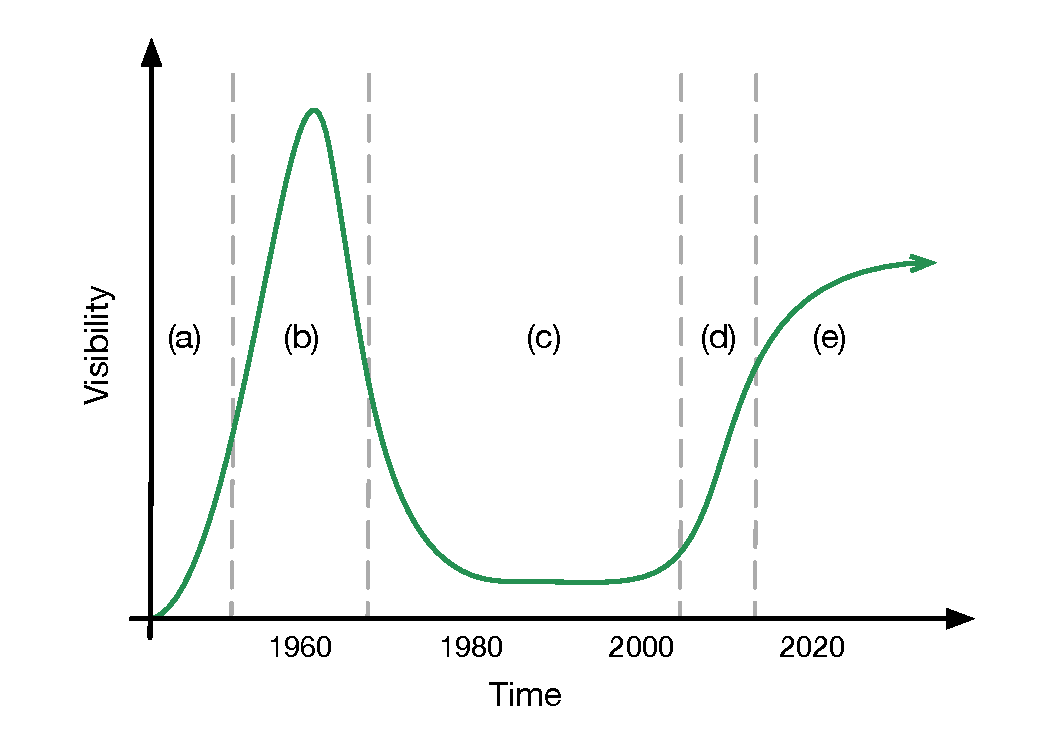
\includegraphics[width=0.6\textwidth]{deephype}
\caption{Gartner Hype cycle, applied to the trajectory of neural networks, consisting of five phases: (a) innovation, (b) peak of inflated expectations, (c) trough of disillusionment, (d) slope of enlightenment, and (e) plateau of productivity.}
\label{fig:deephype}
\end{centering}
\end{figure}

% Deep learning is trending
It goes almost without saying that excitement and interest in deep learning is spiking across computer science, in academia and industry alike.
Research groups are forming based primarily on deep learning, it is being used to win increasing number of data science competitions, and the topic has become common fodder for popular science articles and interviews.
With all the success and attention, it is easy to get carried away in thinking that deep learning is the proverbial ``magic bullet'', that it might topple all problems in due time.

The reality, however, is far more modest.
Deep learning \emph{is} indeed several important things.
It is a powerful approach to non-linear system design.
Deep networks make fantastic models of physical phenomena, and could have profound use in the fields of acoustics, immersive audio, or amplifier modeling.
It is extremely versatile, and can be easily adapted in application-specific ways that other powerful machines, such as SVMs, cannot.
And, given significant gains in compute power, the combination of architectural flexibility and numerical optimization makes it an arguably efficient research strategy, at least more so than graduate students manually tuning parameters.

That said, there are a few important things deep learning is not.
It is by no means the best answer to every problem.
Deep learning is, in its current forms, still relatively data hungry and often computationally expensive.
Even in the case of unsupervised pre-training, sufficient volumes of realistic data may not be trivial to obtain, as in the case of accelerometers or gyroscopes.
To the latter point, any performance gains obtained with a deep network could be effectively negated by disproportionate increase in processing time.
Both of these limitations are like to become less important over time, but remain relevant today.
More conceptually, albeit somewhat contentiously, nor can the modern flavors of deep learning be called ``intelligent'';
echoing the ghost of Searle, a system may certainly \emph{behave} intelligently without truly \emph{being} so.
Despite the imagery evoked by metaphors and figurative language that pervade the field, deep learning has as much in common with humanity as a player piano, and learning is merely a means of programming in a data-driven manner.
This is not to say that deep learning can or will not lead to such breakthroughs, but care should be taken when differentiating metaphor from reality.

% Semantic gap, the limitation of audio signal processing systems whereby the information necessary to make some decision does not truly reside in the signal.
% Wiggins, offers ``the mysterious thing that is Music is an abstract and intangible cultural construct, which does not have physical existence in itself, but which is described by all three of these representational domains'', being the acoustic, the auditory, and the graphemic (notated) \cite{Wiggins2009}.



% Takeaways:
What should one make of deep learning then?
Suffice it to say that deep learning is just another tool ---a powerful tool, but a tool nonetheless--- to be included in the toolbelt of the information science practitioner.
Similar to the trajectories of other, now standard, methods, such as principal components analysis, Gaussian mixture models, or support vector machines, deep learning is settling into the final stage of its hype cycle, the point at which it becomes a means to solve a problem.
\emph{Is deep learning some magic bullet?}
Of course not.
\emph{Is it intelligent?}
Hardly.
But is it useful?
Can it accelerate the process of system design and implementation?
Can it allow the clever researcher to quickly vet ideas and develop complex, robust systems?
The answer to all of these is \emph{yes}.


\subsection{On the Apparent Rise of Glass Ceilings in Music Informatics}

One of the motivating factors of this work was to understand and potentially address the increasing prevalence of diminishing returns in various music description tasks, like chord estimation, genre classification, or mood prediction.
The main hypothesis resulting from an initial survey was the idea that common approaches to system design were inadequate, and another approach to system design, i.e. deep learning, might afford significant performance gains.
However, one of the most significant outcomes of this work is in some sense the most unexpected:
subtle deficiencies in methodology may be contributing as much or more to unsatisfactory results than the algorithms or approaches used to achieve them.

This finding reflects a small but growing trend in music informatics of critically assessing how the scientific method is applied to machine listening tasks, with meta-analyses of genre recognition \cite{Sturm20inf}, rhythmic similarity \cite{Esparza2014}, and music segmentation \cite{Neito2015}, to name a few.
Looking to the intersection of these areas, the research methodology of automatic music description consists of five basic steps:

\begin{enumerate}
\item Define the problem.
\item Collect data.
\item Build a solution.
\item Evaluate the model.
\item Iterate.
\end{enumerate}


With this method as a common underpinning, the evolution of content-based music informatics unfolds logically.
Though a young field, the majority of current research has converged to a handful of established tasks, as evidenced by those conducted at MIREX.
Labeled music data is notorious difficult to amass in large quantities, but resouces have grown steadily for those well-worn problems.
In cases where it has not, researchers are faced with one of two options:
curate the data themselves, or adapt an existing dataset to their problem.
Having developed a solution, it is necessary to benchmark a proposed algorithm against previous efforts.
However, to make such comparisons fairly, it is typically necessary to compute the same metrics over the same data, as the systems themselves are seldom made public.
Thus, most research efforts today focus almost exclusively on (3) and (5), adopting or otherwise accepting the other three.

It is critical to note, though, that these other methodological stages --- problem formulation, data curation, and evaluation--- have developed naturally over time at the community level, based not on globally optimal design but rather a combination of evolving understanding, inertia, and convenience.
At this point, it serves to return to an initial question posed by this work:
why \emph{are} music description systems yielding diminishing returns?
The findings of this work, particularly in the space of automatic chord estimation, corroborate the growing trend that perhaps the biggest problem facing content-based music informatics is one of methodology.

With this in mind, reconsider the case of automatic chord estimation.
What is the scope of the problem being addressed?
``Can an agent provide acceptable chord transcriptions?'' is a very different question from ``Can an agent reproduce \emph{these} chord transcriptions?''
Analysis of the Rock Corpus transcriptions showed that comparing the outputs of two expert musicians can achieve a ``yes'' and ``no'' respectively.
Does the data reflect these requirements?
Chord annotations consist of single perspectives from several anonymized annotators.
It is doubtful that all annotators are using the chord labels the same way.
How do we know when the problem is solved?
Does weighted chord symbol recall with different comparison rules correspond to subjective experience?
Not all substitutions are equal, as the distance in harmonic function between a \texttt{I:7} and a \texttt{I} is quite different from a \texttt{V:7} and a \texttt{V}, for example.

Understandably, it is easy to lose sight of the fact that research is not just the process of iterative system development, but the entire arc of the scientific method.
At this point in the trajectory of music informatics, it is conceivable that several well-worn tasks could use a reassessment of what constitutes methodological best practices.
This is hardly a novel realization, but one that warrants greater awareness within the music informatics community.
% Interestingly enough, it has been over half a decade since Wiggins offered that ``because music is first and foremost a psychological construct, there can be no externally defined truth, and systems which aim to encode musical similarity must, by definition, do so in a human-like way.''
It is necessary, but ultimately insufficient, to tirelessly pursue better solutions;
we must be as dilligent in our pursuit of better problems.


% -------------------------------------------------------------- 
%:                  BACK MATTER: appendices, refs,..
% --------------------------------------------------------------

% the back matter: appendix and references close the thesis


%: ----------------------- bibliography ------------------------

%\clearpage
\onehalfspacing
\bibliographystyle{apacite}

\renewcommand{\bibname}{Bibliography} % changes the header; default: Bibliography

\bibliography{backmatter/library} % adjust this to fit your BibTex file



%: ------ appendices----------------------------------------
\appendix

\chapter{Brownie tootsie roll lollipop cookie}
\label{adx:a}

\doublespacing

Oat cake pudding sweet lemon drops gummies cookie. 
Dragee lollipop ice cream apple pie sweet roll brownie. 
Lollipop marshmallow jelly beans marzipan sugar plum chupa chups caramels toffee. 
Croissant icing chocolate cake oat cake muffin powder tart. 
Croissant wafer dessert pudding cupcake croissant. 
Cheesecake wafer sugar plum danish. 
Liquorice powder sesame snaps.


%: --------------------------- index ---------------------------

%\clearpage
% \begin{footnotesize}
% \cleardoublepage % ensure the right page
% \phantomsection % sets an anchor
% \printindex
% \end{footnotesize}



\end{document}
